\chapter{Implementación}
\label{capitulo5}
\lhead{Capítulo 5. \emph{Implementación}}

En el capitulo anterior realizamos una revisión del estado del arte de los algoritmos de evasión de obstáculos en el contexto de los QUAVs. En este capitulo veremos la descripción de la implementación de la solución propuesta en este trabajo para el problema de evasión de obstáculos sobre el contexto de la plataforma de implementación de los productos de ACSL. En la sección \ref{sec:imp-platform} se describe brevemente la metodología y plataforma de implementación; en la sección \ref{sec:imp-algo} se fundamenta la selección del algoritmo de evasión de obstáculos, uno inspirado en \textit{Learning high-speed flight in the wild} \cite{Loquercio2021}; en la sección \ref{sec:imp-arch} se describe la arquitectura de la solución propuesta en este trabajo, así como también se describe el funcionamiento de cada de sus componentes; y finalmente en la sección \ref{sec:imp-finetune} se describe el proceso de refinamiento fino de la red neuronal encargada de la inferencia de trayectorias libre de colisión, es decir, el refinamiento fino de la política estudiante.

\section{Plataforma de implementación}

\label{sec:imp-platform}

El componente principal de la metodología de implementación de soluciones sobre los productos de ACSL, es una librería propietaria de ACSL llamada \textit{ACSL Vision Core}. Esta librería, escrita en C++, proporciona un marco de trabajo para la implementación de aplicaciones sobre los UAV de ACSL, adicionalmente admitiendo el uso de vehículos simulados por el entorno de simulación AirSim \cite{shah2018airsim}. Bajo este marco de trabajo, una solución es implementada como una colección de procesos de linux independientes que se comunican utilizando memoria compartida y \textit{sockets} de la librería ZeroMQ \cite{zeroMQ}. La implementación del algoritmo a seleccionar debe estar condicionada a este marco de trabajo para que la solución propuesta por este trabajo pueda ejecutarse en concordancia y con capacidad de interacción con otras aplicaciones de los vehículos de ACSL. La libreria \textit{ACSL Vision Core} expone un API (Interfaz de programación de aplicación, del inglés \textit{Aplication Programming Interface}) llamada \textit{ACSL Flight API} que permite interactuar con el FCU del QUAV, exponiendo métodos para leer la información de la estimación del estado del QUAV (posición, velocidad, rotación y estado de los actuadores) y para enviar comandos de control de alto nivel desde un proceso ejecutándose en el computador a bordo del vehículo.

\subsection{Plataforma física}

El vehículo sobre el cual se implementara la solución propuesta en el presente trabajo es SOTEN, un QUAV de tamaño ligero diseñado por ACSL para aplicaciones de fotografía aérea (Inspección, vigilancia, rescate, entre otros). En la figura \ref{fig:SOTEN} se muestra una imagen del vehículo en cuestión.

\begin{figure}[H]
    \centering
    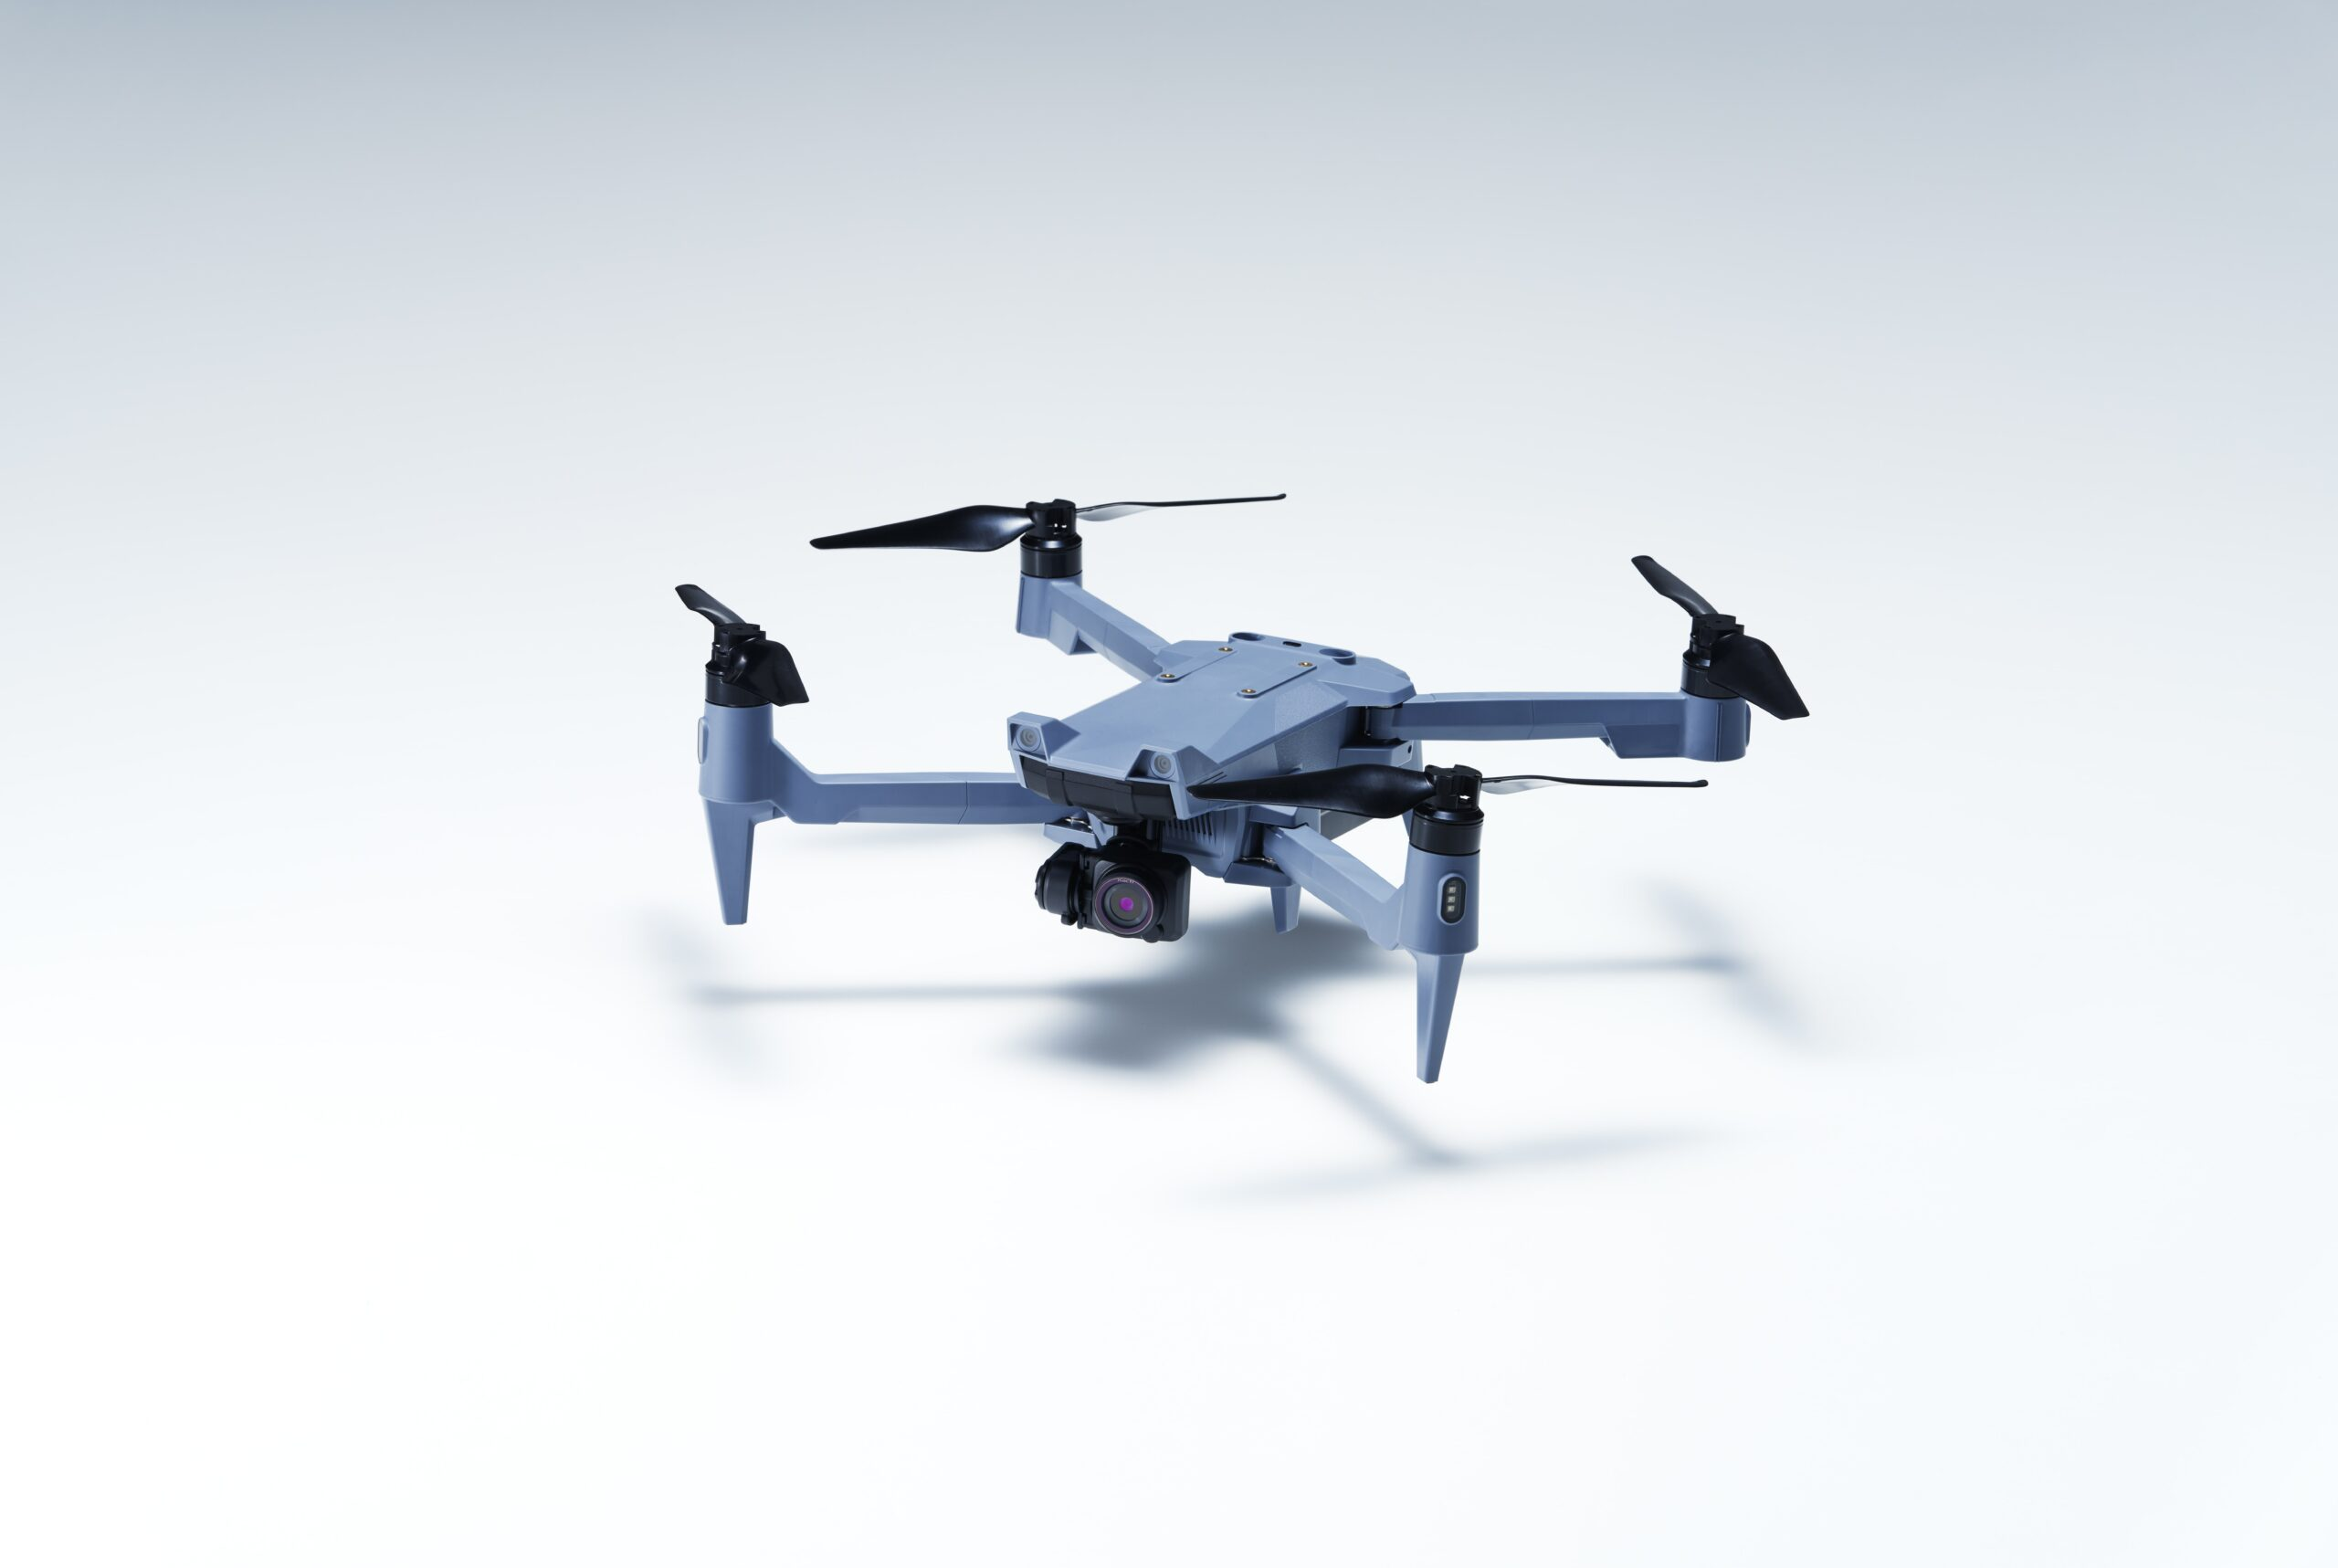
\includegraphics[scale=0.15]{partes/img/SOTEN.jpg}
    \caption[SOTEN, un QUAV diseñado por ACSL que sirve de plataforma física para la implementación de este trabajo.]{SOTEN, un QUAV diseñado por ACSL que sirve de plataforma física para la implementación de este trabajo.}
    \label{fig:SOTEN}
\end{figure}

SOTEN viene equipado con un chip NVIDIA Jetson Xavier NX, que funciona como computadora a bordo del QUAV, que posee capacidades de aceleración gráfica y es precisamente donde se va a implementar la solución propuesta en este trabajo. Con respecto a los sensores, SOTEN viene equipado con un conjunto de cámaras estereoscópicas, de las cuales en este trabajo solo se utilizara el par frontal; así como también se equipa de una cámara de inspección estabilizada por un \textit{gimbal} que si bien no es utilizada en este trabajo, representa una de las funciones principales de SOTEN, su capacidad de inspección. Como mecanismo de localización tiene acceso a locación por GPS y localización por visión, en este trabajo solo se utilizará la localización por GPS. 

\subsection{Entorno de simulación}

El entorno de simulación que es soportado por \textit{ACSL Vision Core} es AirSim \cite{shah2018airsim}, donde se pueden simular una variedad de vehículos equivalentes a los productos de ACSL en entornos de simulación ejecutados por \textit{UnrealEngine}. En este trabajo se utiliza AirSim para simular un QUAV equivalente a SOTEN, que permite que dentro de las simulaciones se tengan las mismas propiedades dinámicas y dimensiones de la plataforma física. La implementación de la solución propuesta en este trabajo es agnóstica de la utilización de AirSim, el \textit{ACSL Flight API} se encarga de traducir los comandos de control al equivalente en el marco de trabajo del simulador.

\section{Selección del algoritmo}

\label{sec:imp-algo}

El algoritmo seleccionado es uno inspirado en el propuesto en \textit{Learning high-speed flight in the wild} \cite{Loquercio2021}. Las características el método propuesto en \cite{Loquercio2021} resultan atractivas para los productos de ACSL, en concreto: solo requiere de la información disponible a bordo del vehículo; no requiere sensores que alguno de los productos de ACSL no tenga disponible; tiene la capacidad de adaptarse a aplicaciones especificas si se escogen adecuadamente los entornos de simulación para la generación de la base datos; como la información visual se representa en forma de un mapa de profundidad, es sencillo trasladar el algoritmo entre plataformas; y finalmente, \cite{Loquercio2021} provee acceso al código fuente para la generación de las base de datos y del entrenamiento de la política estudiante, así como también los pesos entrenados de la red neuronal utilizada en \cite{Loquercio2021}, reduciendo el trabajo necesario para implementar el algoritmo sobre la plataforma de ACSL.

Sin embargo, es necesario realizar ciertas modificaciones al algoritmo. Primero, por motivos de seguridad es necesario que la rapidez de ejecución este limitada a 1 m/s, esto es, \jim{v_{des} = 1}; los pesos de la política estudiante publicados en \cite{Loquercio2021} fueron entrenados con \jim{v_{des} = 7}, por lo tanto es necesario hacer un proceso de ajuste fino de los pesos. Segundo, debido a limitaciones del \textit{ACSL Flight API}, solo se puede enviar instrucciones para modificar la referencia de la velocidad y de la velocidad rotacional; a diferencia de \cite{Loquercio2021} en donde se envían instrucciones con referencia de posición, rotación, velocidad y aceleración simultáneamente, por lo tanto la ejecución de las trayectorias solamente enviará la información de la velocidad lineal junto con un estimado de la velocidad rotacional necesaria para que el encabezado del QUAV apunte hacia la dirección tangencial de la trayectoria en ejecución. Tercero, por motivos de validación del concepto por parte de ACSL, la ejecución de la evasión de obstáculos va a estar limitada al plano \jim{x,y} de marco de referencia del cuerpo del QUAV. En resumen, el algoritmo que se implementa en este trabajo es el mecanismo de inferencia de la política estudiante de \cite{Loquercio2021} luego de un proceso de refinamiento fino; junto con otros componentes implementados dentro del marco de trabajo de ACSL que se encargan de la ejecución de las trayectorias y de la adquisición de la información necesaria para la inferencia.

\section{Arquitectura de la solución}

\label{sec:imp-arch}

Tal como se menciono en la sección anterior, la solución propuesta por este trabajo es la combinación del mecanismo de inferencia de la política estudiante de \cite{Loquercio2021} y una serie de componentes bajo el marco de trabajo de ACSL encargados de la ejecución de las trayectorias y de la adquisición de la información necesaria para la inferencia. La figura \ref{fig:sol-comm} muestra el diagrama de comunicación de la solución propuesta; se compone de cuatro componentes: Un puente del FCU, que se encarga de continuamente obtener la ultima información del estado del QUAV; un puente de profundidad, que procesa los pares de imágenes estéreo producidas por las cámaras frontales para calcular mapas de profundidad; un proceso de inferencia que utiliza la información producida por los puentes de FCU y de profundidad para predecir trayectorias libre de colisión utilizando la red neuronal de \cite{Loquercio2021}; y un ejecutor de trayectorias que ejecuta las trayectorias inferidas por el proceso de inferencia. Los componentes se ejecutan como procesos independientes y se comunican utilizando  \textit{sockets} de la librería ZeroMQ \cite{zeroMQ} y memoria compartida.

\begin{figure}[H]
    \centering
    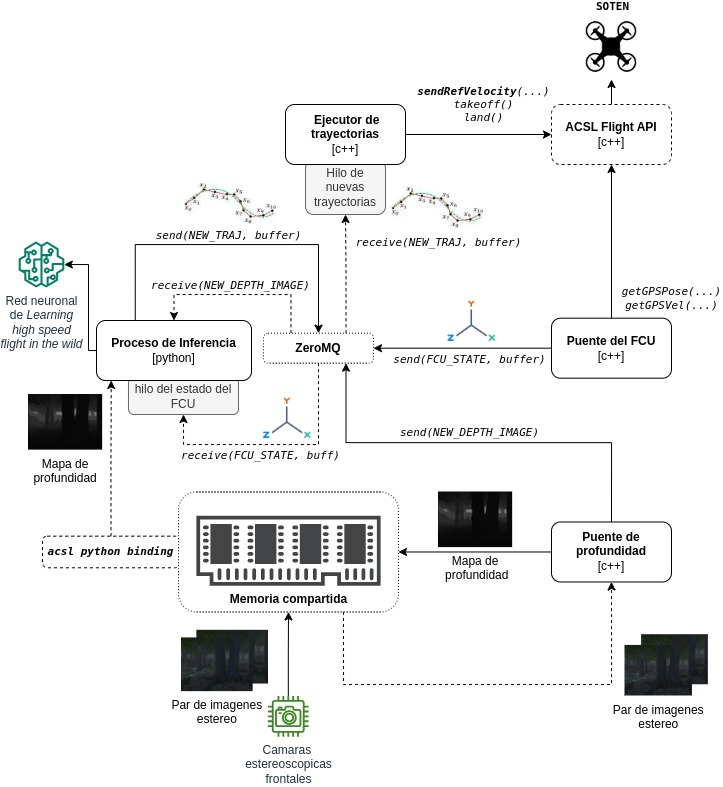
\includegraphics[scale=0.5]{partes/img/Solution-V3-Spanish.jpg}
    \caption[Diagrama de comunicación de la solución.]{Diagrama de comunicación de la solución. En alto nivel, el flujo de información comienza cuando se produce un nuevo par de imágenes estéreo; el puente de profundidad procesa el par para producir un mapa de profundidad; luego el proceso de inferencia recibe el mensaje \texttt{NEW\_DEPTH\_IMAGE}, obtiene la información mas reciente del puente FCU, invoca a la red neuronal y envía el resultado en el mensaje \texttt{NEW\_TRAJ}. Finalmente, el ejecutor de trayectorias, al recibir el mensaje \texttt{NEW\_TRAJ}, proyecta la trayectoria de acuerdo al procedimiento descrito en la sección \ref{sec:prev-aoa-traj} y procede a ejecutar la trayectoria utilizando el \textit{ACSL Flight API}.}
    \label{fig:sol-comm}
\end{figure}

A continuación se profundiza en cada uno de los componentes.

\subsection{Puente del FCU}

Este componente tiene como función obtener la información mas reciente del estado del QUAV y transmitir dicho estado mediante un \textit{socket} de ZeroMQ para su utilización por el proceso de inferencia. Debido a que el proceso de inferencia se ejecuta en python y el \textit{ACSL Flight API} solo esta disponible para entornos de C++, es necesario que un proceso externo obtenga la información del API y se la comunique al proceso de inferencia, esta es justamente la función del puente del FCU.

Si \jim{B} es el marco de refencia del cuerpo del QUAV, a una frecuencia de 120 Hz, este componente invoca las funciones \texttt{getGPSPose} y \texttt{getGPSVel} del \textit{ACSL Flight API} para obtener los estimados mas recientes de: latitud, longitud y altitud (GPS); los ángulos de Euler \textit{roll}, \textit{pitch} y \textit{yaw} de \jim{B}; los componentes \jim{v_{B_x}, v_{B_y}, v_{B_z}} de la velocidad lineal con respecto a \jim{B}; y la velocidad angular del eje \jim{B_z}, \jim{\omega_z}. Adicionalmente, este componte también convierte las coordenadas latitud, longitud, altitud en coordenadas NED utilizando el algoritmo \ref{alg:NED}, tomando como origen al punto de donde despega el QUAV. Finalmente, estas mediciones son empaquetadas en un \textit{buffer} binario y son enviadas como cuerpo del mensaje \texttt{FCU\_STATE} para su posterior uso por el proceso de inferencia.


\subsection{Puente de profundidad}

Este componente es el encargado de generar los mapas de profundidad necesarios para el funcionamiento del proceso de inferencia. Para realizar esta tarea, obtiene el par mas reciente de imágenes estéreo de la cámara frontal, calcula un mapa de disparidad utilizando la funcionalidad de emparejamiento de bloques de la librería \texttt{opencv} \cite{bradski2000opencv}, aplica el método explicado en la sección \ref{sec:teo-stereo} para obtener un mapa de profundidad a partir del mapa de disparidad y constantes de las cámaras; una vez disponible el mapa de profundidad, se escribe en memoria compartida y envía el mensaje \texttt{NEW\_DEPTH\_IMAGE}, que sirve para notificar al proceso de inferencia que hay un nuevo mapa de profundidad disponible. Este proceso se repite con una frecuencia máxima de 30 Hz, que coincide con la tasa de muestreo del sistema de cámaras estéreo frontales de SOTEN.

\subsection{Proceso de inferencia}

Este componente es el encargado de predecir trayectorias libres de colisión a partir de los mapas de profundidad generados por el puente de profundidad y del estado del QUAV obtenido por el puente del FCU. El procesamiento de este componente se divide en dos hilos: el hilo principal, que realiza inferencia en la red neuronal de \textit{Learning High Speed Flight in the Wild} \cite{Loquercio2021} cada vez que llega el mensaje \texttt{NEW\_DEPTH\_IMAGE}; y el hilo del estado del FCU, que se encarga de recibir los mensajes \texttt{FCU\_STATE} para mantener una copia global del ultimo estado del QUAV.

\subsubsection{Hilo del estado del FCU}

El procesamiento realizado por este hilo es relativamente simple; cada vez que llega un mensaje \texttt{FCU\_STATE} se obtiene el \textit{buffer} binario del cuerpo del mensaje, se convierte la representación binaria en una representación estructurada y se le asigna a la variable global \texttt{fcu\_state}. La variable \texttt{fcu\_state}, al ser global, es accesible por ambos hilos. Para mantener la integridad de \texttt{fcu\_state} y evitar condiciones de carrera, el acceso de escritura y lectura esta controlado por un semáforo de exclusión mutua (\textit{mutex}).

\subsubsection{Hilo principal}

El procesamiento del hilo principal puede resumirse en 5 etapas: primero, esperar por un nuevo mensaje de \texttt{NEW\_DEPTH\_IMAGE}; segundo, obtener el ultimo mapa de profundidad de la memoria compartida; tercero, detectar la presencia de obstáculos en el mapa de profundidad, si no existe obstáculo cercano, repetir desde la primera etapa; cuarto, preparar las entradas de la red y realizar inferencia; finalmente, seleccionar las trayectorias que cumplan \jim{c^{*} / c_k \geq 0.95 \, (c^{*} = \min_k c_k)}, codificarlas en un \textit{buffer} binario y enviar un mensaje de \texttt{NEW\_TRAJ} utilizando el \textit{buffer} como cuerpo del mensaje.

La etapa tercera es el resultado de una optimización necesaria para aliviar la carga de procesamiento sobre la computadora a bordo del QUAV. El proceso de realizar inferencia utiliza una porción importante de los recursos de procesamiento del QUAV, si se limita la inferencia exclusivamente a los escenarios donde exista un obstáculo a esquivar, el QUAV puede utilizar los recursos de procesamiento en otras aplicaciones. Para realizar la tarea de detectar obstáculos en un mapa de profundidad, se utiliza un algoritmo que dado un mapa de profundidad retorna un aproximado de la profundidad al obstáculo mas cercano, este algoritmo asume que los obstáculos mas cercanos aparecen mas grandes en el mapa de profundidad y utiliza la funcion \texttt{findContours} de la librería \texttt{opencv} \cite{bradski2000opencv} para obtener los contornos de una máscara binaria. Si \jim{\ell} es la distancia máxima en milímetros donde un obstáculo se considera ``cercano'' y \jim{D} es un mapa de profundidad en milímetros, el pseudo-código del algoritmo se muestra en el algoritmo \ref{alg:nearest-depth}.

\begin{algorithm}
\caption{Pseudo-código del algoritmo para obtener un estimado de la profundidad al obstáculo mas cercano en un mapa de profundidad }
\label{alg:nearest-depth}
\KwData{\jim{D}, \jim{\ell}}
\KwResult{\jim{d}, estimado de la profundidad en metros del obstáculo mas cercano.}

$D_{mask} = D > 10 \wedge D \leq \ell$

\If{$\sum_{(i,j) \in D_{mask}}{D_{mask}(i,j)} > \frac{1}{10} |\{(i,j) \in D\}|$}{
    $\text{\texttt{contornos}} = \text{\texttt{opencv2.findContours(}}D_{mask}\text{\texttt{)}}$ 

    $\text{\texttt{candidato}} = $ el contorno en $\text{\texttt{contornos}}$ con mayor área.

    $a_{cand} = \text{\texttt{candidato.area}}$

    \If{$a_{cand} > \frac{1}{10} |\{(i,j) \in D\}|$}{
        $I_{cont} = \{ (i,j) | (i,j) \in D \wedge (i,j) \in \text{\texttt{candidato}} \}$

        $d = \frac{1}{1000 \cdot |I_{cont}|} \sum_{(i,j) \in I_{cont}}{D(i,j)}$

        \Return{$d$}
    }
}

\Return{\jim{\infty}}

\end{algorithm}

Dicho esto, a continuación se describe el pseudo-código del procedimiento ejecutado por el hilo principal del proceso de inferencia. Dadas las definiciones:

\begin{itemize}
    \item \jim{\Phi: \mathbb{R}^{640 \times 480} \times \mathbb{R}^{15} \longrightarrow \{\mathbb{T}_n |\mathbb{T}_n \text{ es tal como se describe en \ref{sec:aoa-student}}\}} es una función que representa la red neuronal de \textit{Learning High Speed Flight in the Wild} \cite{Loquercio2021}.
    \item \texttt{fcu\_state} es la variable global que contiene el estado mas reciente del QUAV.
    \item \texttt{fcu\_mutex} es el semáforo de exclusión mutua para acceder a \texttt{fcu\_state}.
    \item \jim{\text{\texttt{obs\_distance}}: \mathbb{R}^{640 \times 480} \longrightarrow \mathbb{R^+}} es una implementación del algoritmo \ref{alg:nearest-depth} con \jim{\ell = 7500} mm.
    \item \jim{\text{\texttt{stop}}: \text{\texttt{void}} \longrightarrow \mathbb{B}} es un predicado que indica si el proceso debe terminar.
    \item \jim{\text{\texttt{aplanar}}: \mathbb{R}^{3 \times 3} \longrightarrow \mathbb{R}^{9}} es una función que transforma una matriz 3x3 en el vector resultante de concatenar sus filas en un vector con 9 coordenadas.
    \item \jim{B} representa el marco de referencia en el cuerpo del QUAV.
\end{itemize}

El pseudo-código del procedimiento ejecutado por el hilo principal del proceso de inferencia se muestra en el algoritmo \ref{alg:inference-loop}.

\begin{algorithm}
\caption{Pseudo-código del procedimiento ejecutado por el hilo principal del proceso de inferencia. }
\label{alg:inference-loop}
\KwData{\jim{\Phi}, \texttt{fcu\_state}, \texttt{fcu\_mutex}, \texttt{obs\_distance}, \texttt{stop}}

\While{$\neg \text{\texttt{stop}}()$}{
    Esperar a la llegada de un mensaje de \texttt{NEW\_DEPTH\_IMAGE}.

    Obtener \jim{D}, el mapa de profundidad mas reciente en memoria compartida.

    $d = \text{\texttt{obs\_distance}}(D)$

    \If{$d \leq 7.5$}{
        \Continue
    }

    \texttt{fcu\_mutex.incrementar()}

    Utilizar \texttt{fcu\_state} para obtener \jim{V_B \in \mathbb{R}^{3}}, la velocidad del QUAV con respecto a \jim{B}.

    Utilizar \texttt{fcu\_state} para obtener \jim{q \in \mathbb{R}^{9}}, la rotación de \jim{B} en forma de matriz, esto es, \jim{q = \text{\texttt{aplanar(}}R_{\phi}R_{\theta}R_{\psi}\text{\texttt{)}}} donde \jim{\phi,\theta,\psi} son los ángulos de Euler de B.

    Utilizar \texttt{fcu\_state} para obtener \jim{\mu \in \mathbb{R}^{3}}, posición del QUAV en coordenadas NED.

    Utilizar \texttt{fcu\_state} para obtener \jim{\mu_{goal} \in \mathbb{R}^{3}}, la posición del objetivo del vuelo en coordenadas NED.

    Definir la dirección objetivo como \jim{r = \frac{1}{\|\mu_{goal} - \mu\|}(\mu_{goal} - \mu)}.

    \texttt{fcu\_mutex.decrementar()}

    $X = \text{\texttt{concatenar(}}V_B, q, r\text{\texttt{)}}$

    Realizar inferencia sobre la red neuronal $T = \Phi(D, X)$.

    $c^* = \min \, \{c \, | \, (\tau, c) \in T\}$

    $T_f = \{(\tau, c) \, | \, (\tau, c) \in T \wedge c^* / c \geq 0.95 \}$

    Codificar \jim{T_f} en un \textit{buffer} binario \texttt{traj\_buffer}.

    Enviar mensaje \texttt{NEW\_TRAJ} con \texttt{traj\_buffer} como cuerpo del mensaje.
}

\end{algorithm}

Es importante mencionar, que para que la red neuronal de \textit{Learning High Speed Flight in the Wild} \cite{Loquercio2021} pudiera utilizarse sobre la plataforma de SOTEN, fue necesario realizar un proceso de conversión a un formato ligero orientado a la inferencia. Para esto se utilizó el estándar abierto para la interoperabilidad del aprendizaje de maquinas, ONNX \cite{onnx} (del inglés \textit{Open Standard for Machine Learning Interoperability}). De no haberse realizado esta conversión, el proceso de inferencia podría ejecutarse sobre SOTEN debido a restricciones del \textit{Firmware} del chip NVIDIA Jetson Xavier NX.

\subsection{Ejecutor de trayectorias}

Este componente es el encargado de ejecutar las trayectorias predichas por el proceso de inferencia, así como también manejar el estado de la ejecución del vuelo. El procesamiento de este componente se divide en dos hilos: el hilo de nuevas trayectorias, que recibe los mensajes de \texttt{NEW\_TRAJ} y proyecta las trayectorias en el espacio de los polinomios de grado \jim{N = 3} de acuerdo a lo especificado en \ref{sec:prev-aoa-traj}; y el hilo principal, que ejecuta la trayectoria mas reciente y gestiona el estado del vuelo.

\subsubsection{Hilo de nuevas trayectorias}

Este hilo se encarga de procesar los mensajes de \texttt{NEW\_TRAJ}. Cuando llega un mensaje de \texttt{NEW\_TRAJ}, se decodifica \jim{\mathbb{T}_n = \{ (\tau_{n}^{k}, c_k) | \, 0 \leq k < \beta \}} y \jim{t_{ref}}, con \jim{\beta} siendo el numero de trayectorias que pasaron la selección \jim{c^* / c \geq 0.95} y \jim{t_{ref}} el tiempo en el que se construyo el mensaje, el tiempo \jim{t_{ref}} sirve como referencia al momento de evaluar la trayectoria; luego, por cada \jim{(\tau_{n}^{k}, c_k) \in \mathbb{T}_n}, se proyecta \jim{\tau_{n}^{k}} en el espacio de los polinomios de grado \jim{N = 3} resolviendo el problema de optimización de mínimos cuadrados descrito en la sección \ref{sec:prev-aoa-traj}; posteriormente, a cada proyección \jim{\mu_k} se le escala el tiempo \jim{t} de acuerdo a lo descrito en la sección \ref{sec:prev-aoa-traj} con \jim{v_{des} = 1} m/s; finalmente, se selecciona la proyección con menor costo \jim{c_k} y se le asigna a la variable global \texttt{current\_traj}. La variable \texttt{current\_traj}, al ser global, es accesible por ambos hilos. Para mantener la integridad de \texttt{current\_traj} y evitar condiciones de carrera,  el acceso de escritura y lectura esta controlado por un semáforo de exclusión mutua (\textit{mutex}).

\subsubsection{Hilo principal y máquina de estados}

Este hilo se encarga de la ejecución de la trayectoria actual \texttt{current\_traj} y del manejo del estado del vuelo. Para gestionar el estado del vuelo, utiliza una maquina de estados, la maquina de estados es una estructura que se compone de: un conjunto de estados; una referencia al estado actual; y un espacio de variables compartidas entre estados, tal como el estado del QUAV. Cada estado tiene un identificador, un predicado que indica si se debe entrar a el estado y un procedimiento que se ejecuta en cada iteración que el estado se encuentra como estado actual.

Antes de describir el conjunto de estados de la maquina manejada por el hilo principal, se procede a describir la ejecución guiada por una maquina de estados. En cada iteración: primero, se actualizan las variables compartidas entre estados; segundo, se revisa cuales predicados de transición se cumplen y se modifica el estado actual al estado cuyo predicado de transición se haya cumplido primero; y finalmente, si el QUAV es controlable, se ejecuta el procedimiento del estado actual. 

El hecho de que el QUAV sea controlable depende del operador del vehículo. En el radio control o en la GCS, existe una opción de control que marca al QUAV como no controlable. Cuando un QUAV no es controlable, las instrucciones de alto nivel que se reciben en el FCU desde la computadora a bordo son ignoradas. Esto es simplemente una medida de seguridad que permite que el operador del QUAV pueda manejar manualmente el vehículo en caso de que la ejecución autónoma produzca algún riesgo de colisión o accidente.

Volviendo a la ejecución guiada por una maquina de estados, dadas las definiciones:

\begin{itemize}
    \item \jim{\text{\texttt{stop}}: \text{\texttt{void}} \longrightarrow \mathbb{B}} es un predicado que indica si el proceso debe terminar.
    \item \jim{\text{\texttt{controlable}}: \text{\texttt{void}} \longrightarrow \mathbb{B}} es un predicado que indica si el QUAV es controlable.
    \item \texttt{M} es una maquina de estados tal como se describió anteriormente, con \texttt{M.shared} el espacio de las variables compartidas entre estados, \texttt{M.states} el conjunto de estados y \texttt{M.current\_state} una referencia al estado actual.
    \item Si \texttt{s} es un estado tal como se describió anteriormente. \texttt{s.pred} es el predicado de transición del estado, que recibe el identificador del estado actual y una referencia al espacio de variables compartidas; \texttt{s.proc} es el procedimiento de ejecución, que recibe una referencia al espacio de variables compartidas; y \texttt{s.id} es el identificador del estado.
\end{itemize}

El pseudo-código del procedimiento de ejecución guiada por una maquina de estados se muestra en el algoritmo \ref{alg:state-machine-exec}.

\begin{algorithm}
\caption{Pseudo-código del procedimiento de ejecución guiada por una maquina de estados. }
\label{alg:state-machine-exec}
\KwData{\texttt{stop}, \texttt{controlable}, \texttt{M}}

\While{$\neg \text{\texttt{stop}}()$}{
    Actualizar las variables de \texttt{M.shared}. En este caso, se utilizan las funciones \texttt{getGPSPose} y \texttt{getGPSVel} del \textit{ACSL Flight API} para actualizar el estado del QUAV. 

    \For{\texttt{s} $\in$ \texttt{M.states}}{
        \If{\texttt{s.pred(M.current\_state.id, M.shared)}}{
            \texttt{M.current\_state} $=$ \texttt{s}

            \Break \textbf{linea 3}
        }
    }

    \If{\texttt{controlable()}}{
        \texttt{M.current\_state.proc(M.shared)}
    }
}

\end{algorithm}

Ahora que el concepto de ejecución guiada por maquina de estado esta claro, solo basta con conocer el conjunto de estados, sus transiciones y sus procedimientos de ejecución para comprender el funcionamiento del hilo principal. La figura \ref{fig:state-machine} muestra una visualización de la maquina de estados que guía la ejecución del hilo principal, podemos observar sus identificadores y sus predicados de transición. A continuación se describe cada uno de los estados de la figura \ref{fig:state-machine}. 

\begin{figure}[H]
    \centering
    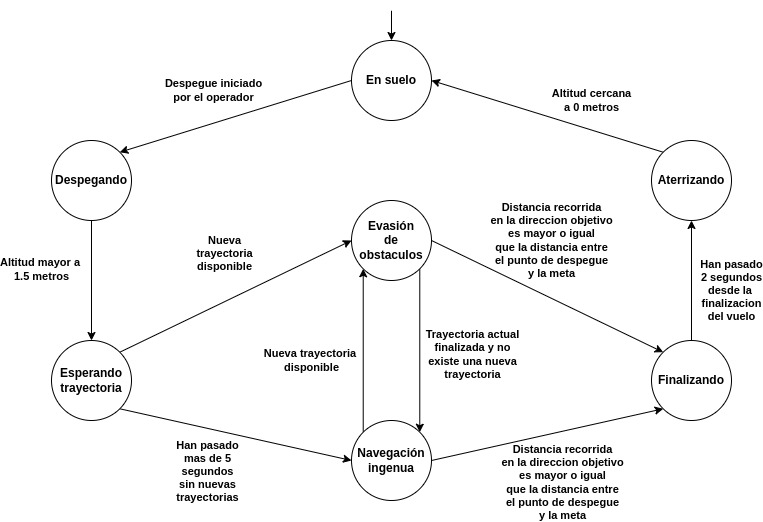
\includegraphics[scale=0.54]{partes/img/State Machine.jpg}
    \caption[Visualización de la maquina de estados que guía la ejecución del hilo principal del ejecutor de trayectorias.]{Visualización de la maquina de estados que guía la ejecución del hilo principal del ejecutor de trayectorias. Los nodos del grafo dirigido representan los estados, sus lados las transiciones y el texto asociado a cada lado representa el predicado de transición.}
    \label{fig:state-machine}
\end{figure}

El estado ``En suelo'' es el estado inicial de la maquina de estados, representa el momento en el que QUAV esta en suelo, bien sea porque se esta preparando para despegar o porque acaba de completar un aterrizaje. El estado ``Despegando'' esta activo durante el proceso despegue, el proceso de despegue comienza cuando el operador del QUAV inicia la secuencia de despegue, bien sea manualmente o de forma autónoma. Una vez que el vehículo alcanza una altitud de 1.5 metros o mayor, el estado ``Esperando trayectoria'' se activa; este estado espera a que se genere una trayectoria, esto es, que el proceso de inferencia envié el mensaje \texttt{NEW\_TRAJ} y que dicho mensaje se procese por el hilo de nuevas trayectorias, en otras palabras, este estado espera a que \texttt{current\_traj} este definido. Luego, si pasados cinco segundos aun no se genera una trayectoria, el estado ``Navegación ingenua'' se activa; en caso contrario, el estado ``Evasión de obstaculos'' se activa.

Los estados ``Evasión de obstaculos'' y ``Navegación ingenua'' son los estados mas importantes para la ejecución del vuelo evadiendo obstáculos. En resumen, el estado ``Evasión de obstaculos'' ejecuta la trayectoria mas reciente generada por el proceso de inferencia y el estado ``Navegación ingenua'' navega directamente en dirección a \jim{\mu_{goal}}, la meta. Recordando que el proceso de inferencia envía nuevas trayectorias siempre y cuando hayan obstáculos a esquivar; el estado ``Evasión de obstaculos'' se activa cuando es necesario evadir un obstáculo y el estado ``Navegación ingenua'' se activa cuando no hay obstáculos cercanos en la dirección objetivo. 

El procedimiento de ejecución del estado ``Navegación ingenua'' es bastante simple, se obtiene la dirección objetivo, se le multiplica \jim{v_{des} = 1} m/s la rapidez de ejecución deseada, y se invoca la función \texttt{sendRefVelocity} del \textit{ACSL Flight API} para que el QUAV navegue directamente en esa dirección. Recordando que \jim{B} es el sistema de referencia del cuerpo del QUAV y \jim{E} es el sistema de referencia inercial; la función \texttt{sendRefVelocity} permite especificar \jim{\omega_{B_z}} la velocidad rotacional alrededor del eje \jim{z} de \jim{B}. Este estado, además de especificar la velocidad, estima la cantidad \jim{\omega_{B_z}} necesaria para que el encabezamiento del QUAV y la dirección objetivo estén en la misma linea. Dicho esto, El pseudo-código del procedimiento de ejecución del estado ``Navegación ingenua'' se muestra en el algoritmo \ref{alg:naive-execution}.

\begin{algorithm}
\caption{Pseudo-código del procedimiento de ejecución del estado ``Navegación ingenua''. }
\label{alg:naive-execution}
\KwData{\texttt{acslFlightApi}, \texttt{M.shared}, \jim{v_{des}}}

Obtener \texttt{fcu\_state} de \texttt{M.shared}.

Utilizar \texttt{fcu\_state} para obtener \jim{\mu \in \mathbb{R}^{3}}, posición del QUAV en coordenadas NED.

Utilizar \texttt{fcu\_state} para obtener \jim{\mu_{goal} \in \mathbb{R}^{3}}, la posición del objetivo del vuelo en coordenadas NED.

Definir la dirección objetivo como \jim{r_E = \frac{1}{\|\mu_{goal} - \mu\|}(\mu_{goal} - \mu)}.

Estimar la velocidad angular instantánea alrededor del eje \jim{B_z} para alinear el encabezamiento del QUAV con \jim{r_E}, esto es \jim{\omega_{B_z} = \arctan(r_{E_y}, r_{E_x}) - \psi } donde \jim{\psi} es el ángulo \textit{yaw} del vehículo.

Utilizar \texttt{fcu\_state} para obtener la matriz de transformación entre \jim{E} y \jim{B}, esto es \jim{R_{E}^{B} = R_{\phi}R_{\theta}R_{\psi}} donde \jim{\phi,\theta,\psi} son los ángulos de Euler de B. 

Obtener la dirección objetivo con respecto a \jim{B}, \jim{r_B = R_{E}^{B} r_E}.

Definir la nueva velocidad, \jim{V_{B} = v_{des} \cdot r_B}

$\text{\texttt{acslFlightApi.sendRefVelocity(}}V_{B}, \omega_{B_z}\text{\texttt{)}}$

\end{algorithm}

Por otro lado, el procedimiento de ejecución del estado ``Evasión de obstaculos'' evalúa la proyección polinómica de la trayectoria actual \texttt{current\_traj} para obtener la velocidad instantánea, posteriormente invoca \texttt{sendRefVelocity} para enviar la referencia de la velocidad y de \jim{\omega_{B_z}} al FCU. Si \texttt{traj\_mutex} es el semáforo de exclusión mutua para el acceso a \texttt{current\_traj}, el pseudo-código del procedimiento de ejecución del estado ``Evasión de obstaculos'' se muestra en el algoritmo \ref{alg:traj-execution}.

\begin{algorithm}
\caption{Pseudo-código del procedimiento de ejecución del estado ``Evasión de obstaculos''. }
\label{alg:traj-execution}
\KwData{\texttt{acslFlightApi}, \texttt{M.shared}, \texttt{current\_traj}, \texttt{traj\_mutex}}

Obtener el tiempo actual del sistema \jim{t_{now}} en segundos.

\texttt{traj\_mutex.incrementar()}

Obtener \jim{t_{ref}} de \texttt{current\_traj} en segundos.

$dt = t_{now} - t_{ref}$

\If{$dt > 1$}{
    Trayectoria completada, \texttt{traj\_mutex.decrementar()} y \Return
}

Obtener $a_x, a_y$ los coeficientes de la proyección polinómica de \texttt{current\_traj} para los ejes \jim{x,y} respectivamente.

$T^\prime = [0, 1, 2dt, 3dt^2]$

$v_x = a_{x}^T \cdot T^\prime$

$v_y = a_{y}^T \cdot T^\prime$

\texttt{traj\_mutex.decrementar()}

Por motivos de validación de concepto, se limita la ejecución de las trayectorias inferidas al plano \jim{B_xB_y}, esto es \jim{v_z = 0}.

$V_{B} = [v_x, v_y, v_z]^T$

Obtener \texttt{fcu\_state} de \texttt{M.shared}.

Utilizar \texttt{fcu\_state} para obtener la matriz de transformación entre \jim{B} y \jim{E}, esto es \jim{R_{B}^{E} = (R_{E}^{B})^T = (R_{\phi}R_{\theta}R_{\psi})^T} donde \jim{\phi,\theta,\psi} son los ángulos de Euler de B. 

$V_{E} = R_{B}^{E} V_{B}$

Estimar la velocidad angular instantánea alrededor del eje \jim{B_z} para que el encabezamiento del QUAV apunte hacia la dirección tangencial de la trayectoria, esto es \jim{\omega_{B_z} = \arctan(V_{E_y}, V_{E_x}) - \psi } donde \jim{\psi} es el ángulo \textit{yaw} del vehículo.

$\text{\texttt{acslFlightApi.sendRefVelocity(}}V_{B}, \omega_{B_z}\text{\texttt{)}}$

\end{algorithm}

Tanto el estado ``Navegación ingenua'' como el estado ``Evasión de obstaculos'' tienen una transición al estado ``Finalizando'', esta transición se cumple cuando cuando la distancia recorrida en la dirección objetivo es mayor o igual que la distancia entre el punto de despegue y la meta; esta condición se utilizó para preferir que el QUAV aterrice si la evasión de obstáculos lo desvió considerablemente de camino original, así como también para que se aterrice una vez que se alcanzo la meta. Dependiendo de la configuración de los obstáculos, es posible que no sea posible avanzar hacia la meta sin desviarse considerablemente, esta transición se asegura de que en ese caso se aterrice el vehículo y se termine el vuelo. En términos formales, trabajando en el sistema de coordenadas NED, si \jim{\mu_0} es posición del QUAV después del despegue y antes de comenzar la navegación; \jim{\mu} es la posición actual del QUAV; y \jim{\mu_{goal}} es la posición de la meta. Esta transición se cumple si la expresión de la ecuación \ref{eq:finishing-condition} se evalúa a verdadero.

\begin{equation}
    \label{eq:finishing-condition}
    (\mu - \mu_0)^T \cdot \left (\frac{\mu_{goal} - \mu_0}{\|\mu_{goal} - \mu_0\|}  \right) \geq \|\mu_{goal} - \mu_0\|
\end{equation}

El estado ``Aterrizando'' se activa una vez que han pasado dos segundos desde que activó el estado ``Finalizando'', este estado invoca al método \texttt{land} del \textit{ACSL Flight API} para ordenar al FCU que aterrice el QUAV de forma autónoma. Una vez que que la altitud es cercana a cero metros, se activa una vez mas el estado ``En suelo'' y la ejecución finaliza.

Es importante mencionar que esta maquina de estados fue diseñada para el caso donde se hace un solo vuelo, en donde el objetivo se encuentra a distancia predefinida en la dirección del encabezado del QUAV al momento del despegue. Para aplicaciones donde exista una secuencia de puntos objetivos sera necesario utilizar una variante de esta maquina de estados en donde se tome en cuenta la secuencia de vuelo. 

\section{Ajuste fino de la política estudiante}

\label{sec:imp-finetune}

Para que las trayectorias generadas por el proceso de inferencia cumplan con la restricción de poder ejecutarse a una rapidez promedio de \jim{v_{des} = 1} m/s; es necesario realizar un ajuste de los pesos de la red neuronal publicada por \cite{Loquercio2021}. Los pesos que se descargaron del repositorio de \textit{Learning High Speed Flight in the Wild} fueron entrenados con una base de datos de trayectorias con \jim{v_{des} = 7} m/s. Por lo tanto, siguiendo las recomendaciones de los autores de \cite{Loquercio2021}, para obtener una política estudiante que sea capaz de evadir obstáculos a una velocidad considerablemente inferior, es necesario realizar un proceso de ajuste fino de los pesos provistos. Según \cite{Loquercio2021}, entrenar una política estudiante requiere de una base de datos extensa de trayectorias generadas por el experto privilegiado, esto acompañado de un tiempo de entrenamiento considerable; es por esto que un su lugar, recomiendan ajustar el conocimiento de la política estudiante que ejecuta con \jim{v_{des} = 7} m/s en lugar de entrenar desde cero.

Para realizar este ajuste fino, se utilizó la plataforma de generación de base de datos del experto informado publicada en el repositorio de \cite{Loquercio2021}. Luego de ajustar la velocidad de ejecución del experto a \jim{v_{des} = 1} m/s, se procedió a generar una base de datos de trayectorias libres de colisión dentro del entorno de ``bosque denso'', que justamente es el entorno principal utilizado en \cite{Loquercio2021} y que consiste en un bosque con arboles cuya posición se determina por una distribución aleatoria de \textit{poisson} \cite{Loquercio2021}. Se realizaron 193 simulaciones, cada una generando entre 300 y 350 ejemplos. De esas 193 simulaciones, se tomaron 168 para formar una base de datos de entrenamiento y 25 para una base datos de validación; en otras palabras, se particionó la base de datos en \jim{~88\%} conjunto de entrenamiento y \jim{~12\%} conjunto de validación.

Se realizo entrenamiento supervisado con la base de datos generada por un total de 33 épocas; comenzando desde la época en el que se encontraba el punto de control de los pesos publicados por \cite{Loquercio2021}, la época numero 188; hasta la época numero 221. Por limitaciones de memoria del computador de entrenamiento, el valor del tamaño del \textit{batch} se redujo de 8 a 1. El valor del resto de los los hiper-parámetros del entrenamiento fueron los mismos utilizados por \cite{Loquercio2021} para la época 188.

\section{Resumen}

En este capítulo, se detalla la implementación de la solución propuesta para abordar el problema de evasión de obstáculos en el contexto de los QUAVs. Comenzamos presentando la metodología y la plataforma de implementación en la sección \ref{sec:imp-platform}, destacando la infraestructura utilizada para desarrollar y evaluar la solución. En la sección \ref{sec:imp-algo}, justificamos la elección del algoritmo de evasión de obstáculos, basándonos en el enfoque presentado en \textit{Learning high-speed flight in the wild} \cite{Loquercio2021}.

La sección \ref{sec:imp-arch} se dedica a la descripción detallada de la arquitectura de la solución propuesta, incluyendo el funcionamiento de cada uno de sus componentes. Aquí, se profundiza en los aspectos cruciales de la ejecución de la solución, en donde destacan el funcionamiento del proceso de inferencia y del ejecutor de trayectorias. Finalmente, en la sección \ref{sec:imp-finetune}, se explora el proceso de refinamiento fino de la red neuronal encargada de la inferencia de trayectorias libre de colisión, es decir, el perfeccionamiento de la política estudiante.

Este capítulo sienta las bases para la evaluación del desempeño de la solución propuesta, que se abordará en el próximo capítulo. El análisis detallado de la implementación proporciona una comprensión completa de la estructura y funcionamiento de la solución, preparando el terreno para la discusión de resultados y conclusiones.